\documentclass[11pt]{article}

\usepackage{minted,xcolor}
\usemintedstyle{monokai}
\definecolor{bg}{HTML}{282828}
\usepackage{xcolor, colortbl}
\usepackage{graphicx}
\usepackage{titlesec}
\usepackage[hmargin=2cm,vmargin=2.5cm]{geometry}
\usepackage{fancyhdr}
\usepackage{hyperref}
\usepackage{caption}
\usepackage{subcaption}

\definecolor{tableaublue}{RGB}{78, 121, 167}

\hypersetup{
    colorlinks=true,
    linkcolor=black,
    filecolor=tableaublue,      
    urlcolor=tableaublue,
    pdftitle={Overleaf Example},
    pdfpagemode=FullScreen,
}

\setlength\parindent{0cm}
\setlength\headheight{28pt}

\titleformat{\section}{\normalfont\Large\bfseries}{Part~\thesection:}{6pt}{}[{\titlerule[0.5pt]}]
\titleformat{\subsection}{\normalfont\large\bfseries}{Exercise~\thesubsection:}{6pt}{}

\graphicspath{ {./img/} }

% \title{Practical’s instruction – Networks (week 7)}
% \author{CSC3833 - Data Visualization and Visual Analytic}

\begin{document}

\pagestyle{fancy}
\renewcommand{\headrulewidth}{0pt}
\fancyhead[L]{CSC8626/CSC8642 - Data Visualization}
\fancyhead[R]{2023 / 2024}
\fancyfoot[L]{\thepage}
\fancyfoot[C]{}
\fancyfoot[R]{School of Computing, Newcastle University}

\begin{center}
\vspace*{1cm}
{\textbf {\Huge Practical 3}}\\
\vspace*{0.5cm}
{\textbf {\huge Time Series and Maps}}
\vspace*{1cm}
\end{center}

\section{Car sales}
% ----------------------------------------------------------------------------------------------------------------

Part one of the assignment consists of providing a representation for analyzing car registrations data over time to identify patterns, trends, and changes, using time series representations.

\subsection*{Data}

This assignment relies on a vehicle registrations dataset from the Department for Transport (DFT). It contains information on Ultra Low Emission Vehicles (ULEVs) registered since 2001.\\
Source: \href{https://www.gov.uk/government/collections/vehicles-statistics}{Vehicle Licensing Statistic}\\

\underline{File}: CarSalesData\_NorthEast.xls\\
This file is available on the Canvas page of the module, which can be accessed at \href{https://ncl.instructure.com/courses/49730}{link}.\\

\underline{Parameters}:
\begin{table}[h!]
    \centering
    \begin{tabular}{|l|m{8cm}|}
        \hline
        Period & period of time \\
        \hline
        Cars & number of cars registered \\
        \hline
        Motor cycles & number of motor cycles registered \\
        \hline
        Light goods & number of light goods registered \\
        \hline
        Heavy goods & number of heavy goods registered \\
        \hline
        Buses \& coaches & number of buses \& coaches registered \\
        \hline
        Other vehicles & number of other vehicles registered \\
        \hline
        Total & total number of vehicles registered \\
        \hline
        Year-on-year change in total vehicles &  \\
        \hline
        Average CO2 emissions for newly registered cars &  \\
        \hline
        Ultra Low Emission Vehicles (ULEVs) & number of ULEVs registered among all vehicles \\
        \hline
        Ultra Low Emission Cars (ULEVs) & number of ULEVs registered among cars \\
        \hline
        Plug in Grant Eligible cars and Vans &  \\
        \hline
        Plug in Non Grant Eligible cars and Vans &  \\
        \hline
    \end{tabular}
    % \caption{Parameters contained within the dataset}
    % \label{tab:my_label}
\end{table}

\subsection{Car registration data dashboard}

Design a one-page interactive dashboard illustrating the fluctuations in car registration since 2001 and how they compare to ULEVs registered during the same period.\\

The dashboard should provide users with the capability to compare the amount vehicles registered over time depending on their body type. It should allow users to discern recurring registration patterns and, lastly, assist them in identifying the ULEVs marketplace.\\

Tips:
\begin{itemize}
    \item Labels such as 'Sum of' can be edited under 'Visualizations' $>$ 'Build Visual' $>$ 'Y-axis' $>$ \textit{arrow down} $>$ 'Rename for this visual' (see Figure \ref{fig:rename}).
    \item If you are using colours to encode categorical information, remember to keep the colours consistent throughout the entire dashboard and avoid reusing the same hue to encode other information.
\end{itemize}

\begin{figure}[h!]
    \centering
    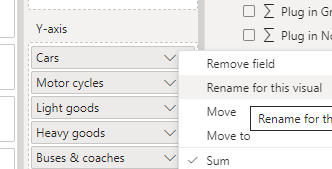
\includegraphics[width=.4\linewidth]{img/rename.png}
    \caption{Renaming a label}
    \label{fig:rename}
\end{figure}

Don't forget to seek feedback from a demonstrator once you have completed your work.\\

\underline{Expected results}:

\begin{figure}[h!]
    \centering
    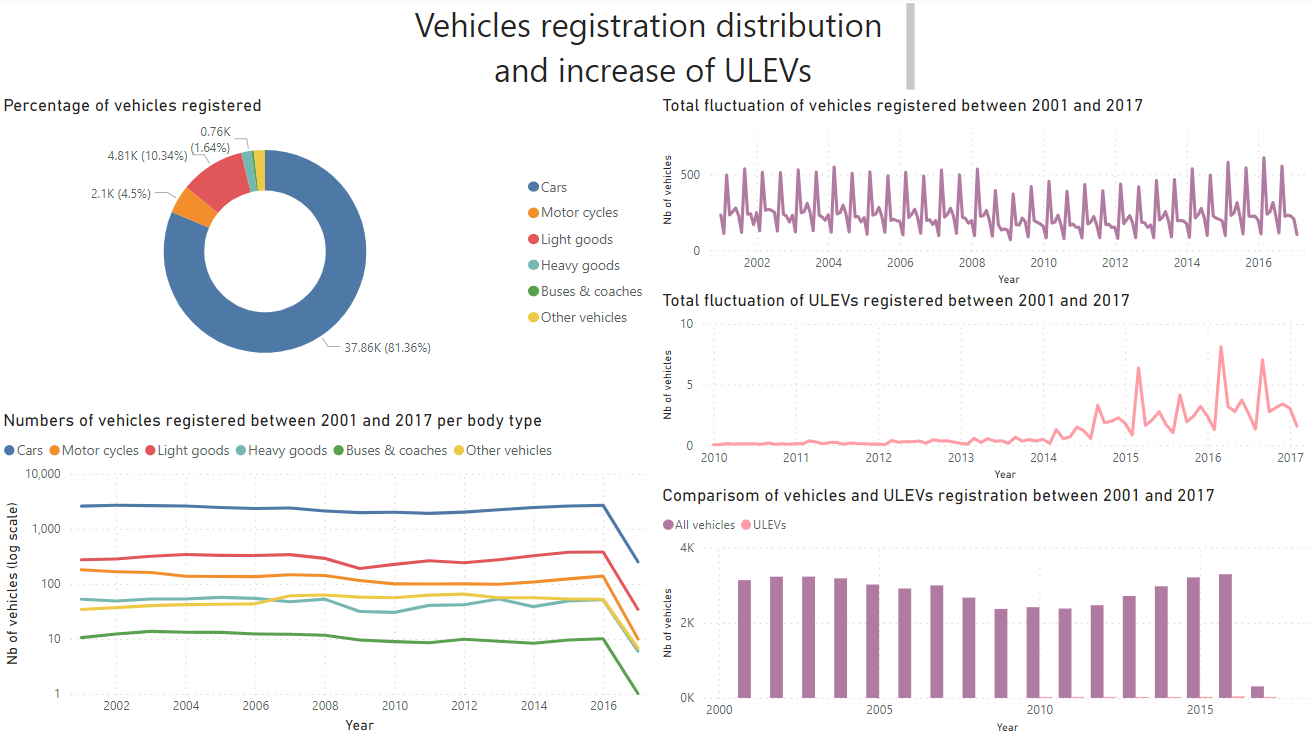
\includegraphics[width=\linewidth]{img/overallCar.png}
\end{figure}

\clearpage

\section{Maps}
% ----------------------------------------------------------------------------------------------------------------

Part two of the assignment consists of providing a representation for exploring deprived areas of Cambridgeshire based on different indicators (domains and sub-domains).

\subsection*{Data}

This assignment relies on two different files:
\begin{itemize}
    \itemsep0em 
    \item The indices of deprivation of Cambridgeshire
    \item The localisation of Lower-layer Super Output Areas (LSOA).
\end{itemize}

The English indices of deprivation measure of Cambridgeshire contains relative levels of deprivation in 32,844 small areas or neighbourhoods, called Lower-layer Super Output Areas (LSOA). This file contains the deprivation ranks and deciles for each LSOA for the six sub-domains and their three respective domains. LSOA with a rank of 1 is the most deprived and the LSOA with a rank of 32,844 is the least deprived.\\
\\
The six sub-domains, and their respective domains, are as follows:

\begin{itemize}
    \item The \textbf{education, skills and training deprivation domain} measures the lack of attainment and skills in the local population
    \begin{itemize}
        \item The \textbf{children and young people sub-domain} measures the attainment of qualifications
        \item The \textbf{adult skills sub-domain} measures the lack of qualifications in the resident working-age adult population
    \end{itemize}
    \item The \textbf{barriers to housing and services domain} measures the physical and financial accessibility of housing and local services
    \begin{itemize}
        \item The \textbf{geographical barriers sub-domain} relates to the physical proximity of local services
        \item \textbf{wider Barriers sub-domain} includes issues relating to access to housing such as affordability
    \end{itemize}
    \item The \textbf{living environment deprivation domain} measures the quality of the local environment
    \begin{itemize}
        \item The \textbf{indoors sub-domain} measures the quality of housing
        \item The \textbf{outdoors sub-domain} contains measures of air quality and road traffic accidents
    \end{itemize}
\end{itemize}
Source: \href{https://data.cambridgeshireinsight.org.uk/dataset/indices-deprivation}{Cambridgeshire Insight - Indices of deprivation}\\

The localization file contains the latitude and longitude of all the LSOAs of England.\\
    
\underline{Files}: DeprivationDomains\_Cambridgeshire.xslx \& GeographicLocalisation\_England.csv\\
These files are available on the Canvas page of the module, which can be accessed at \href{https://ncl.instructure.com/courses/49730}{link}.\\

\underline{Parameters}:

\begin{table}[h!]
    \centering
    \begin{tabular}{|l|m{9cm}|}
        \hline
        LSOA code (2011) & LSOA identifier \\
        \hline
        LSOA name (2011) & LSOA name \\
        \hline
        Local Authority District code (2019) & region identifier \\
        \hline
        Local Authority District name (2019) & region name \\
        \hline
        $<$\textit{domain or sub-domain}$>$ Rank & LSOA rank for the relative domain or sub-domain \\
        \hline
        $<$\textit{domain or sub-domain}$>$ Decile &  LSOA decile for the relative domain or sub-domain \\
        \hline
    \end{tabular}
    \caption{Deprivation file parameters}
    \label{tab:Deprivation}
\end{table}

\begin{table}[h!]
    \centering
    \begin{tabular}{|l|m{13cm}|}
        \hline
        LSOA11CD & LSOA identifier \\
        \hline
        LSOA11NM & LSOA name \\
        \hline
        BNGEAST & LSOA east localisation according to the British National Grid (BNG) \\
        \hline
        BNGNORTH & LSOA north localisation according to the BNG \\
        \hline
        LONGITUDE & LSOA longitude \\
        \hline
        LATITUDE & LSOA latitude \\
        \hline
    \end{tabular}
    \caption{Localisation file parameters}
    \label{tab:Localisation}
\end{table}

\subsection{Deprived areas of Cambridgeshire}

Compare the most deprived (ranked under 3000) to least deprived (ranked above 3000) location of Cambridgeshire for at least three sub-domains.\\

Create one page of visuals for each sub-domain. On each page should contains two maps (most and least deprived location) and use one numerical slicer per map to interact with the ranges.\\

Tips:
\begin{itemize}
    \item To connect the data in the localisation file and in the deprivation file, identify their common parameters and associate them with each other. Go to 'Table View' $>$ 'Manage Relationship' $>$ 'New' and link the common parameters in both tables (see Figure \ref{fig:relation}).
    \item To display only the LSOA of Cambridgeshire use the 'Filter' panel (see Figure \ref{fig:filter}).
    \item To assign a slicer to a map click on the slicer than 'Format' $>$ 'Edit interactions' and select the associated map only (see Figure \ref{fig:interaction}).
    \item Copy and paste will be useful in completing this. You can duplicate whole pages, just right click on the page tab.
\end{itemize}

\begin{figure}[h!]
    \centering
    \begin{minipage}{.5\textwidth}
      \centering
    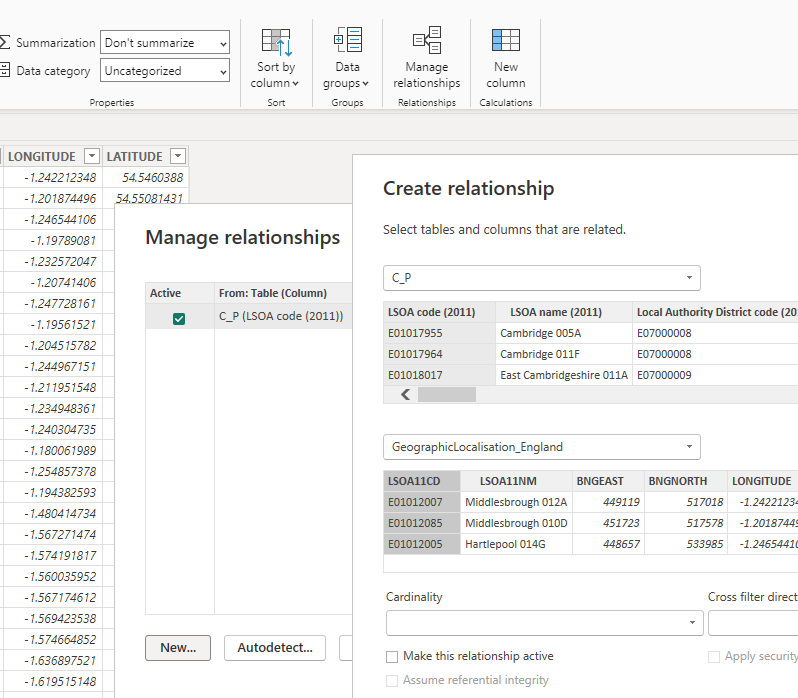
\includegraphics[width=.7\linewidth]{img/relation.png}
      \captionof{figure}{Associate parameters from different files}
      \label{fig:relation}
    \end{minipage}%
    \begin{minipage}{.5\textwidth}
      \centering
      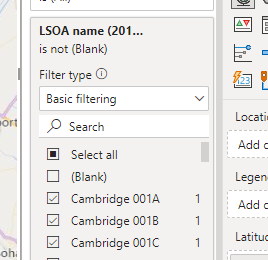
\includegraphics[width=.6\linewidth]{img/filter.png}
      \captionof{figure}{Filter LSOA}
      \label{fig:filter}
    \end{minipage}
\end{figure}

\begin{figure}[h!]
    \centering
    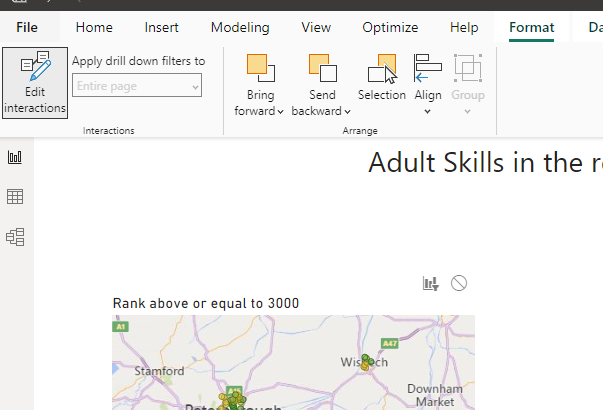
\includegraphics[width=.4\linewidth]{img/interaction.PNG}
    \caption{Assign a slicer to a map}
    \label{fig:interaction}
\end{figure}

\clearpage

\underline{Expected results}

\begin{figure}[h!]
    \centering
    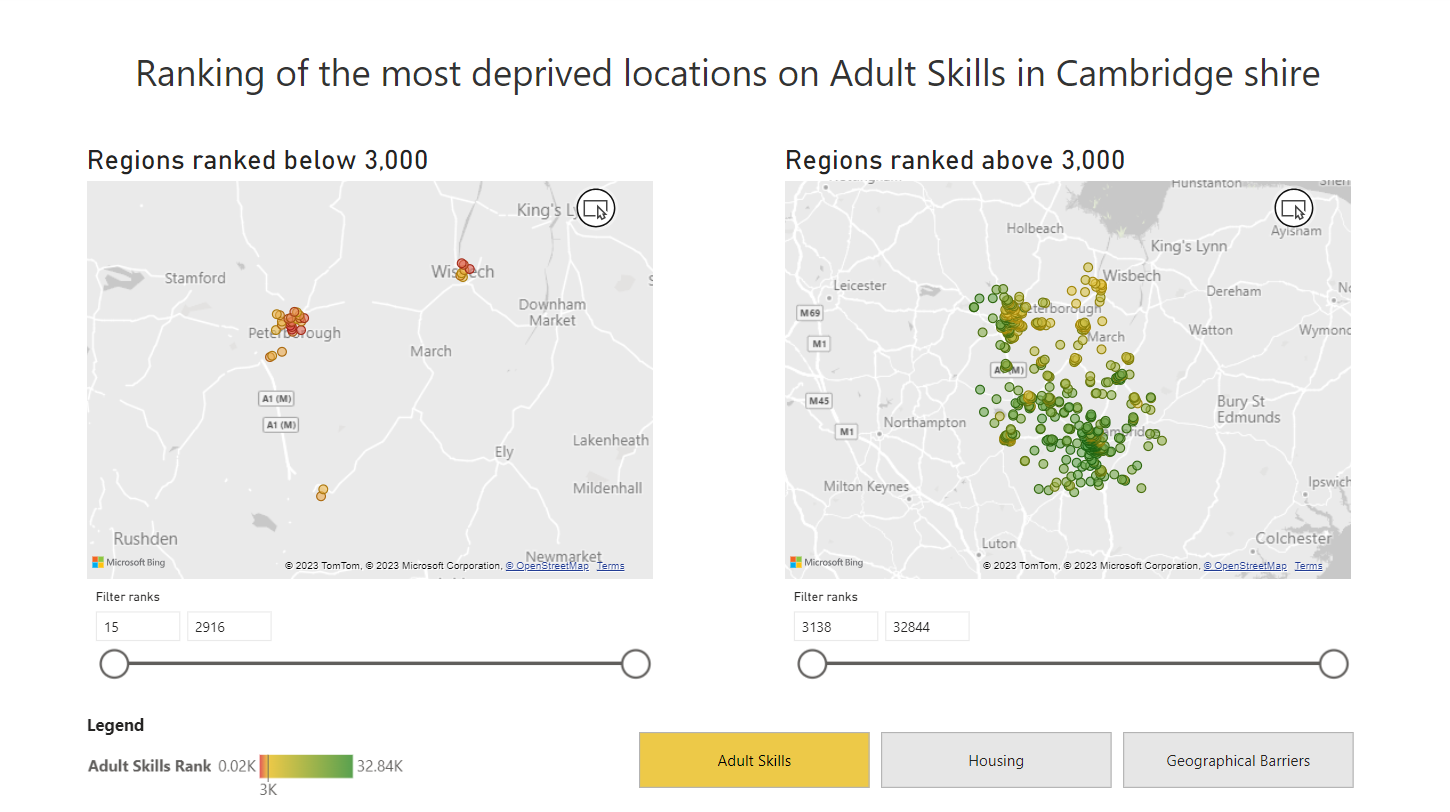
\includegraphics[width=\linewidth]{img/practicalmap.png}
    % \caption{Expected result for the exercise 1.1}
    % \label{fig:overallCar}
\end{figure}

\end{document}